\chapter{Din\'amica}
\label{cha:dinamica}

\section{Primera Ley de Newton}

\subsection{Transformaciones de Galileo}

La velocidad y la aceleraci\'on dependen del sistema de referencia usado para el c\'alculo de los mismos. Considere dos sistemas de referencia en movimiento relativo: $x,y,z,t$ y $x',y',z',t'$. Como el tiempo es absoluto
\begin{align}
  t=t'\qquad v\ll c\,.
\end{align}
Sea $\mathbf{r}$ el vector de posici\'on de un cuerpo relativo al primer sistema de referencia, y $\mathbf{r}'$ su vector de posici\'on relativo al segundo. Asumiendo que los sistema de referencia coinciden en el tiempo $t=t'=0$, entonces
\begin{align}
  \mathbf{r}(t)=\mathbf{r}'(t)+\mathbf{R}(t)\,.
\end{align}
donde el sistema de coordenadas primado se mueve con velocidad $\mathbf{V}$ a largo de $\mathbf{R}$:
\begin{align}
  \mathbf{R}(t)=\mathbf{V}\, t\,,
\end{align}
donde $d\mathbf{V}/dt=0$. Entonces
\begin{align}
  \mathbf{r}=&\mathbf{r}'+\mathbf{V}t\nonumber\\
  \mathbf{r}'=&\mathbf{r}-\mathbf{V}t\,.
\end{align}

En el caso especial de un sistema de referencia movi\'endose a lo largo del eje $x$, tenemos
\begin{align}
  \mathbf{r}'=\mathbf{r}-V t\hat{\mathbf{i}}\,,
\end{align}
o
\begin{align}
  t'=&t\nonumber\\
  x'=&x-vt\nonumber\\
  y'=&y\nonumber\\
  z'=&z\,.
\end{align}
\begin{align}
  \begin{pmatrix}
    t'\\
    x'\\
    y'\\
    z'\\
  \end{pmatrix}=
  \begin{pmatrix}
    1&0&0&0\\
    -V&1&0&0\\
    0&0&1&0\\
    0&0&0&1\\
  \end{pmatrix}
  \begin{pmatrix}
    t\\
    x\\
    y\\
    z\\
  \end{pmatrix}
\end{align}
Como la velocidad $\mathbf{V}$ no cambia con el tiempo:
\begin{align}
  \mathbf{v}'(t)=\mathbf{v}(t)-\mathbf{V}\,.
\end{align}
Pero para la aceleraci\'on:
\begin{align}
  \mathbf{a}'=\mathbf{a}\,.
\end{align}


\subsection{Primera Ley}

Un objeto se mueve uniformemente en el espacio siempre y cuando no hayan influencias externas actuando sobre \'el.

El movimiento tiene sentido solamente con respecto a un sistema particular de coordenadas, y al momento de describir el movimiento es esencial especificar el sistema de coordenadas que se este usando. Un sistema de coordenadas inercial, es un sistema de coordenadas que se mueve a velocidad constante.

\textbf{Primera Ley de Newton}: Los cuerpos aislados se mueven uniformemente en sistemas inerciales.

Un cuerpo sobre el que no act\'uan fuerzas se llama \emph{cuerpo libre}.

\section{Principios de la Mecánica}
La homogeneidad e isotropía del espacio, y la homogeneidad del tiempo permiten son ejemplos de transformaciones continuas que forman lo que matemáticamente se conocen como Grupos de Lie. 

\textbf{Principio de relatividad:} Las leyes de la física mantienen su forma en distintos sistemas inerciales.

Las cantidades físicas pueden sufrir transformaciones de traslaciones o rotaciones bajo grupos continuos, pero las leyes físicas deben mantener su forma después de estas transformaciones. Más aún, \textbf{El Teorema de Noether} establece que por cada transformación continua existe alguna carga conservada. En mecánica este teorema da lugar a tres leyes de conservación importantes, resumidas en la Tabla~\ref{tab:tn}

\begin{frame}
  
\begin{table}
  \centering
  \begin{tabular}{|l|l|l|}\hline{}
    \textbf{Transformación} &\textbf{Ley Física}  &  \textbf{Cantidad conservada}\\\hline
Traslaciones espaciales & Principio de moméntum & Moméntum\\
Traslación temporal & Principio de Energía & Energía\\
Rotaciones & Principio de momentum angular & Moméntum angular\\\hline
  \end{tabular}
  \caption{Implicaciones del teorema de Noether en mecánica}
  \label{tab:tn}
\end{table}
\end{frame}

En este curso estableceremos y usaremos cada uno de estos tres principios.

\section{Principio de Moméntum}

Primero algunas definiciones:

\subsection{Sistema y entorno}

Un \emph{sistema} puede estar conformada por uno o más objetos. Todo lo que no está incluido en el sistema es parte del \textbf{entorno}



\subsection{Segunda Ley de Newton}

\begin{frame}
  %\begin{block}%
{El Principio de Moméntum}, que también se conoce como la Segunda Ley de Newton es:
\begin{align}
  \Delta\mathbf{p}=\mathbf{F}_{\text{neta}}\Delta t
\end{align}
  %\end{block}
\end{frame}
%Falta discusión de la notas del cuaderno aquí


Las fuerza neta actuando en un sistema en un instante es el vector de
suma de todas la fuerzas ejercida sobre el sistema por todos los
objetos del entorno, las cuales son llamadas fuerzas externas. Puede
haber fuerzas internas al sistema, ejercidas por un objeto del sistema
en otro objeto del sistema, pero tales fuerzas internas no pueden
cambiar el moméntum del sistema. Veremos luego en detalle por qué en
el siguiente capítulo, pero la idea básica es que las fuerzas internas
se cancelan entre si. Una fuerza que el objeto 1 hace sobre el objeto
2 en el sistema cambia el moméntum del objeto 2, pero el objeto 2
ejerce una fuerza en dirección opuesta en el objeto 1 que cambia el
moméntum del objeto de la forma opuesta, de modo que el cambio en el
moméntum de los dos objetos suma cero.




  

\begin{frame}
  \begin{block}%
{Pregunta:} Una bola cayendo hacia la tierra consiste de muchos
  átomos. Cada átomo en la bola ejerce fuerzas en sus átomos vecinos
  de la bola, la tierra ejerce fuerzas en cada átomo de la bola, y el
  aire ejerce fuerzas en los átomos de la superficie de la
  bola. Tomando la bola como el sistema, y la tierra y el aire como el
  entorno, ¿cuales de estas fuerzas son externas y cuales internas?.
    
  \end{block}

  
\end{frame}

\begin{frame}
\begin{itemize}
  \item     \alert{La tierra y el aire} son parte del entorno, de modo que las fuerzas
    ejercidas por la tierra el aire son ambas \alert{externas}.
  \item Las fuerzas\alert{inter-atómicas} de los átomos de la bola son
    fuerzas \alert{internas} que no contribuyen a la fuerza neta $\mathbf{F}_{\text{neta}}$
  \end{itemize}
  
\end{frame}

\begin{frame}
  La cantidad de interacción afectando un objeto incluye tanto la \alert{intensidad de la interacción} ($\mathbf{F}_{\text{neta}}$) y la \alert{duración} $\Delta t$ de la interacción. Un mayor cambio de moméntum es causado bien sea por una fuerza más grande o por aplicar la fuerza durante más tiempo.
\end{frame}

\begin{frame}
  %\begin{block}%
{Definición de impulso:}
\begin{align}
  \text{Impulso}=\mathbf{F}_{\text{neta}}\Delta t
\end{align}
en unidades SI de $\text{N}\cdot\text{s}$ (newton-segundo)
  %\end{block}
\end{frame}

Con esta definición del impulso podemos establecer el Principio de Moméntum en las siguientes palabras:
\begin{frame}
  \begin{center}
    \textbf{El cambio de moméntum de un sistema es igual al impulso aplicado a éste.}
  \end{center}
\end{frame}

Ejemplo: Una fuerza constante de $(3,-5,4)\ $N actúa en un objeto durante $10\ $s. ¿Cuál es el impulso neto aplicado al objeto? ¿Cual fue el cambio en el momentum del objeto?
\begin{align}
\text{Impulso}=\mathbf{F}_{\text{neta}}\Delta t=(3,-5,4)\ \text{N}\cdot (10\ \text{s})=
(30,-50,40)\ \text{N}\cdot\text{s}\,.
\end{align}
El cambio en el moméntum del objeto es igual al impulso neto, de modo que
\begin{align}
  \Delta \mathbf{p}=(30,-50,40)\ \text{Kg\,m/s}
\end{align}


\begin{frame}
  \begin{figure}
    \centering
%\only<1>{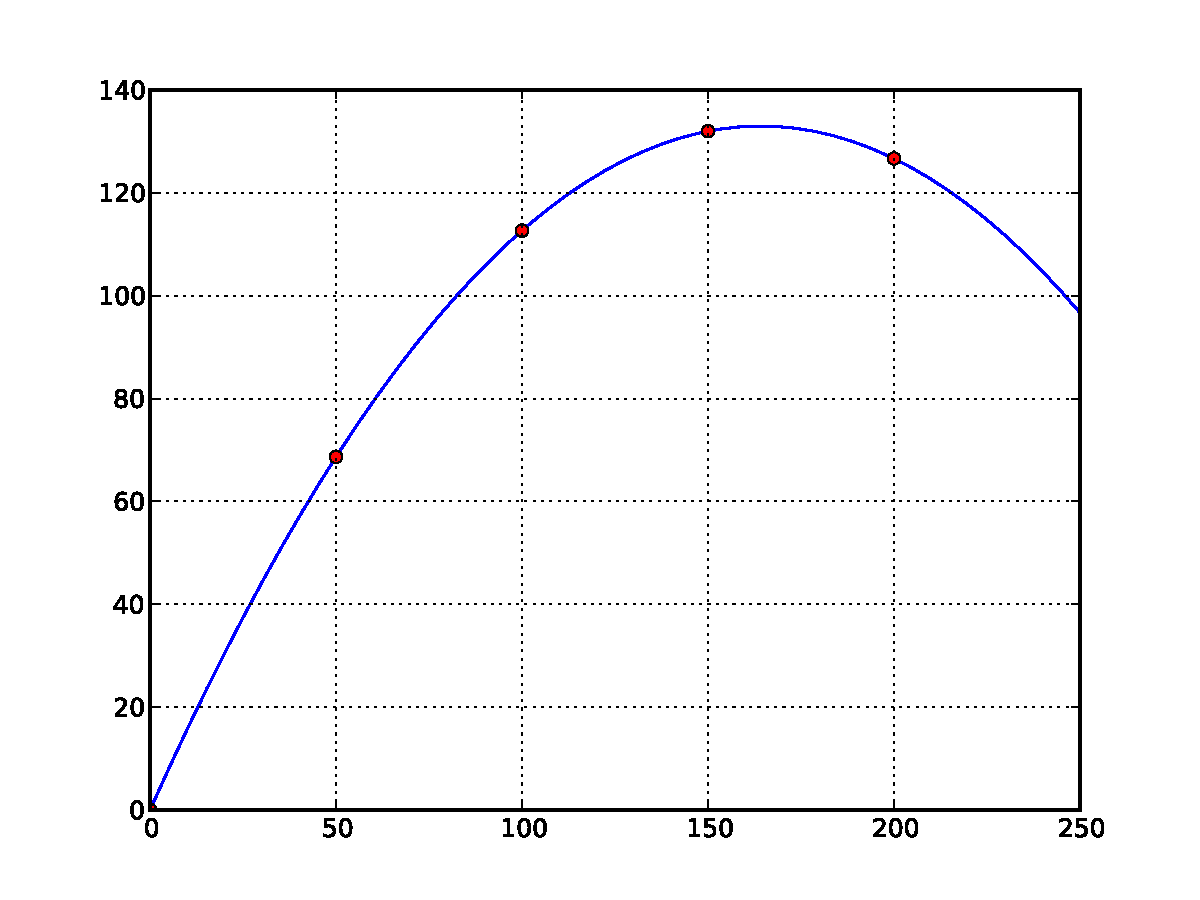
\includegraphics[scale=0.5]{trayectoria1}}%
%\only<2>{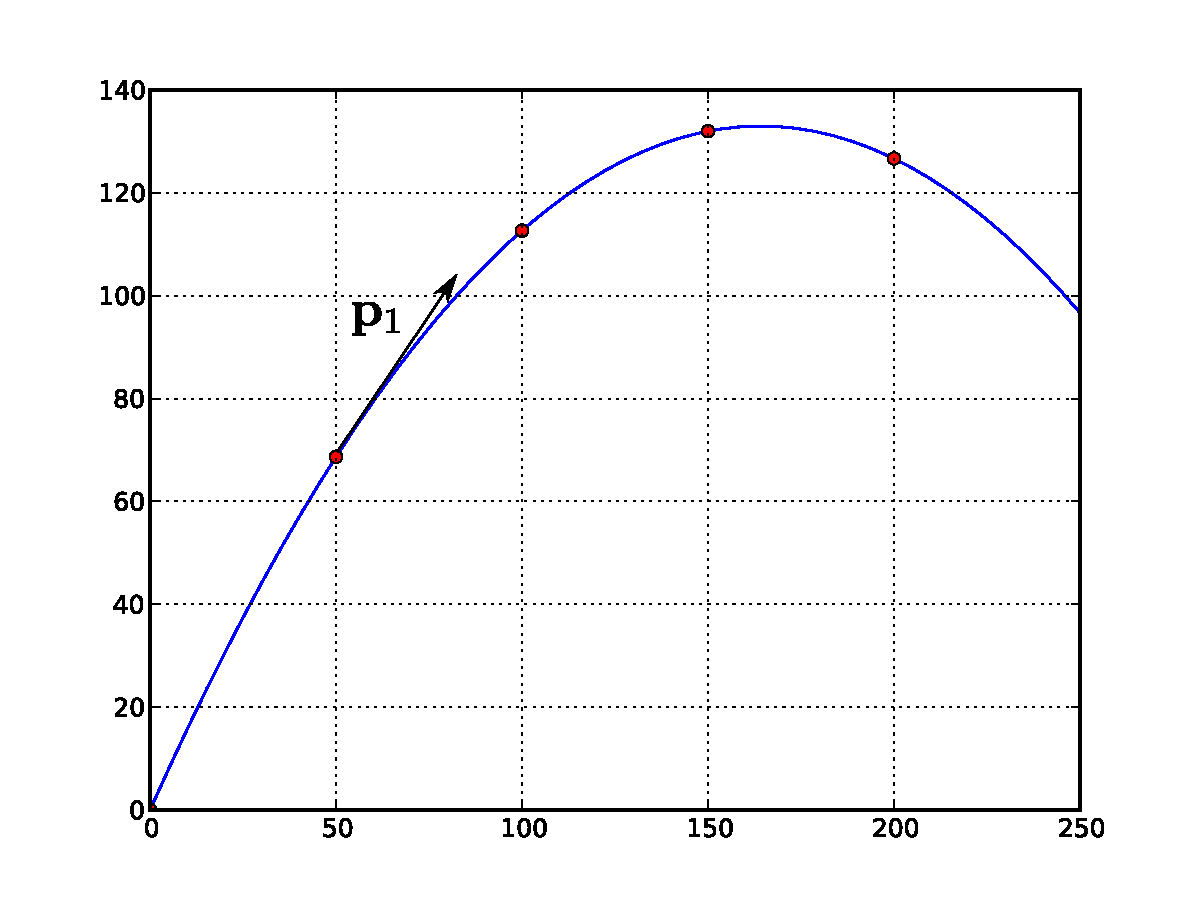
\includegraphics[scale=0.5]{trayectoria2}}%
%\only<3>{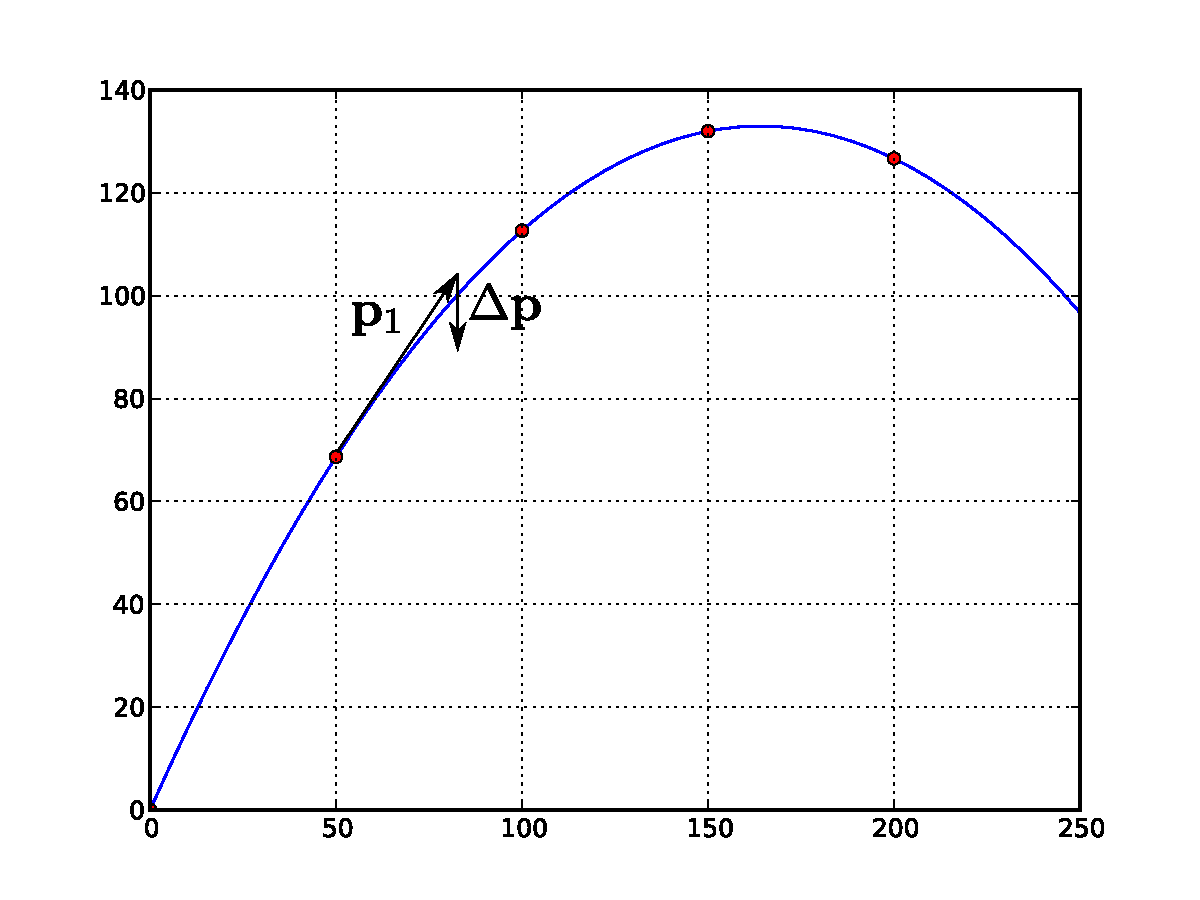
\includegraphics[scale=0.5]{trayectoria3}}%
%\only<4>{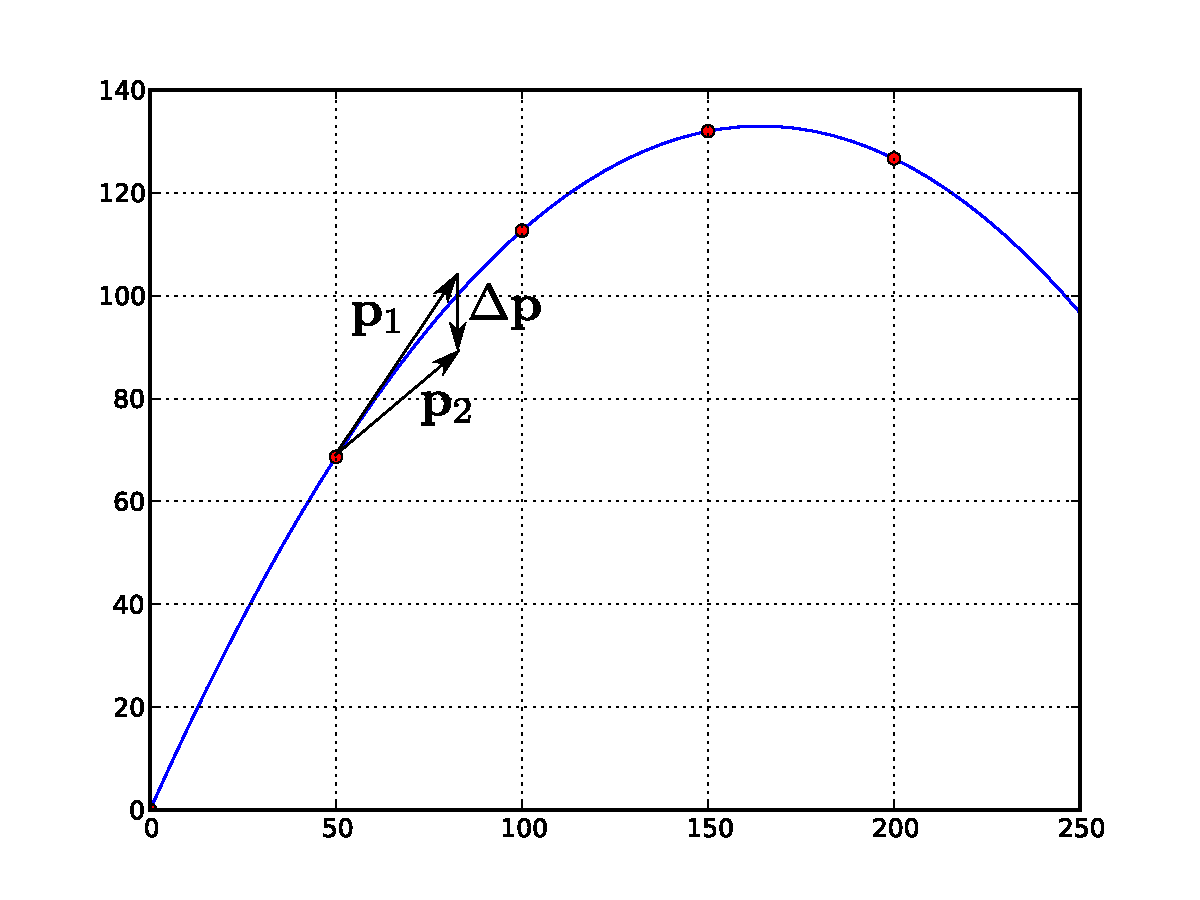
\includegraphics[scale=0.5]{trayectoria4}}%
%\only<5>%
{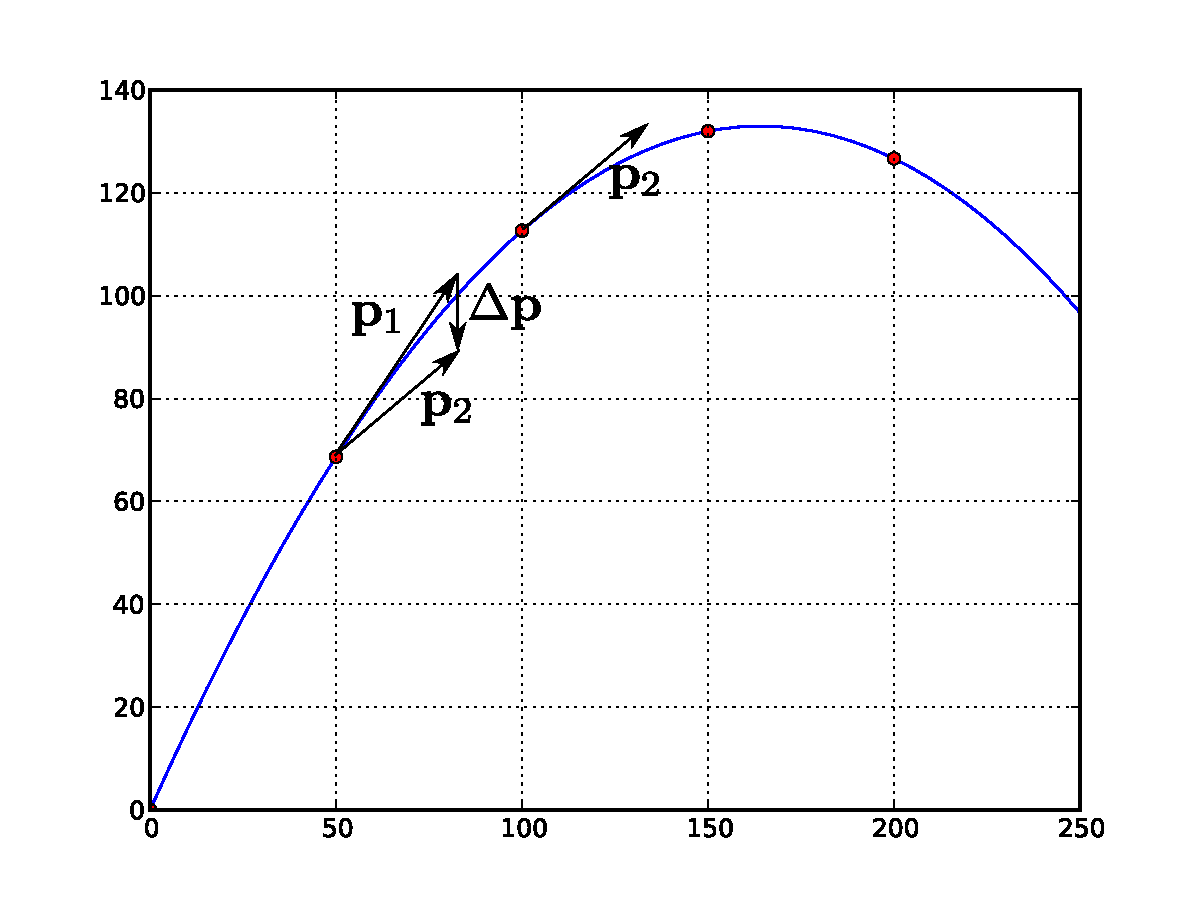
\includegraphics[scale=0.5]{trayectoria5}}
    \caption{Actualización del momentun}
    \label{fig:1}
  \end{figure}
\end{frame}

El proceso iterativo que se puede implementar computacionalmente equivale a hacer la integral sobre la ecuación de movimiento dada por el Principio de Momentum. Sin embargo, sólo en casos muy específicos se puede realizar analíticamente la integración de la ecuación de movimiento.


Como para un $\Delta t$ infinitesimal, la fuerza siempre se puede considerar constante, el principio de momentum se puede reescribir como
\begin{align}
  \label{eq:28}
  \mathbf{F}_{\text{neta}}=&\lim_{\Delta t\to 0}\frac{\Delta\mathbf{p}}{\Delta t}\nonumber\\
 \mathbf{F}_{\text{neta}}=&\frac{d\mathbf{p} }{dt}
\end{align}
Si $\mathbf{F}_{\text{neta}}$ es conocida, a la ec.~\eqref{eq:28}, se conoce como ecuación de movimiento.

\begin{frame}
  \begin{block}%
{Ecuación de movimiento:}
  \begin{align*}
   \mathbf{F}_{\text{neta}}=&\frac{d\mathbf{p} }{dt}
   \end{align*}
  \end{block}
\end{frame}

\subsection{Caso especial: masa constante}
En el caso especial en que la masa del sistema, $m$, es constante, la ecuación de movimiento puede reescribirse como
\begin{align}
   \mathbf{F}_{\text{neta}}=&\frac{d m\mathbf{v} }{dt}\nonumber\\
   \mathbf{F}_{\text{neta}}=&m\frac{d \mathbf{v} }{dt}\nonumber\\
   \mathbf{F}_{\text{neta}}=&m\mathbf{a}\,.
\end{align}

\begin{frame}
  \begin{block}%
{Caso especial: masa constante}
\begin{align}
   \mathbf{F}_{\text{neta}}=&m\mathbf{a}\,.
\end{align}
\end{block}
\end{frame}

\subsection{Caso especial: Fuerza y masa constante}

Si la fuerza neta es constante en dirección y magnitud en el caso de masa constante, la ecuación de movimiento puede integrarse analíticamente. Para simplificar el análisis consideremos una fuerza neta constante sólo con componente en $x$:
\begin{align}
  \mathbf{F}_{neta}=(F_x,0,0)\,.
\end{align}

La ecuación de movimiento se reduce a
\begin{align}
  a_x=&\frac{F_x}{m}\nonumber\\
\frac{dv_x}{dt}=&\frac{F_x}{m}\nonumber\\
{dv_x}=&\frac{F_x}{m}{dt}\,.
\end{align}
Integrando a ambos lados de la igualdad, desde un tiempo inicial $t_i$ a un tiempo final $t$, con $v_{xi}=v_x(t_i)$ y $v_x=v_x(t)$, tenemos
\begin{align}
  \int_{v_{xi}}^{v_x} d v_x =&\int_{t_i}^t \frac{F_x}{m}{dt}\nonumber\\
  v_x-v_{xi} =&\frac{F_x}{m}\int_{t_i}^t {dt}\nonumber\\
\end{align}

\begin{align}
  \label{eq:36}
  v_x =&v_{xi}+\frac{F_x}{m}(t-t_i)\,,
\end{align}

\begin{align}
  \frac{dx}{dt} =&v_{xi}+\frac{F_x}{m}(t-t_i)\nonumber\\
  {dx} =&v_{xi}{dt}+\frac{F_x}{m}(t-t_i){dt}\,,
\end{align}
e integrando de nuevo con $x_i=x(t_i)$ y $x=x(t)$, tenemos
\begin{align}
  \int_{x_i}^{x}{dx} =&v_{xi}\int_{t_i}^t{dt}+\frac{F_x}{m}\int_{t_i}^t{dt}(t-t_i){dt}\,,
\end{align}

Haciendo $u=t-t_i$, $du=dt$, obtenemos
\begin{align}
\int(t-t_i)dt=\int u du=\frac{1}{2}u^2=\frac{1}{2}(t-t_i)^2\,,
\end{align}
de modo que
\begin{align}
  x-x_i=&v_{xi}(t-t_i)+\frac{F_x}{m}\left.\frac{1}{2}(t-t_i)^2\right|^t_{t_i}
\end{align}
\begin{align}
  x=&x_i+v_{xi}(t-t_i)+\frac{1}{2}\frac{F_x}{m}
  \left[
    (t-t_i)^2-(t_i-t_i)^2
  \right]\nonumber\\
  x=&x_i+v_{xi}(t-t_i)+\frac{1}{2}\frac{F_x}{m}(t-t_i)^2
\end{align}
\begin{frame}
  \begin{block}%
{Solución analítica:} al problema de movimiento en una dimensión bajo la influencia de una fuerza constante
\begin{align}
   x=&x_i+v_{xi}(t-t_i)+\frac{1}{2}\frac{F_x}{m}(t-t_i)^2
\end{align}
  \end{block}
\end{frame}


Un ejemplo de fuerza constante, es la fuerza gravitacional sobre un objeto de masa $m$ que se encuentra cerca a la superficie de la tierra:
\begin{align}
  \label{eq:29}
  \mathbf{F}_{\text{grav}}=(0,F_y,0)\approx(0,-mg,0).
\end{align}
El signo menos índica que la fuerza va dirigida hacía la superficie de la tierra, donde hemos establecido el origen de coordenadas

Si dicho cuerpo cae libremente desde una altura $y_i$ desde la superificie de la tierra, y con una velocidad $v_{yi}$, la ecuación para su altura $y$ desde un origen de coordenadas sobre la superficie de la tierra es
\begin{align}
\label{eq:31}
   y=&y_i+v_{yi}(t-t_i)+\frac{1}{2}\frac{F_y}{m}(t-t_i)^2\nonumber\\
   y=&y_i+v_{yi}(t-t_i)-\frac{1}{2}g(t-t_i)^2\,.
\end{align}
mientras que para la componente de la velocidad en $y$, tenemos de la ec.~\eqref{eq:36}
\begin{align}
  \label{eq:37}
    v_y =&v_{yi}-g(t-t_i)\,,
\end{align}

\begin{frame}
  \begin{block}%
{Solución analítica:} al problema de caida libre en la dirección $y$ perpendicular a la superficie de la tierra y con origen de coordenadas sobre la superficie de la tierra:
\begin{align*}
     y=&y_i+v_{yi}(t-t_i)-\frac{1}{2}g(t-t_i)^2\nonumber\\
     v_y =&v_{yi}-g(t-t_i)\nonumber\\
     a_y=&-g\,.
\end{align*}

  \end{block}
\end{frame}


\subsection{Ecuación de la trayectoria}
Para un cuerpo en movimiento vertical bajo la influencia de una fuerza gravitacional constante, tenemos que si la rapidez inicial es $v_0$ para una altura inicial $y_0$, entoces de \eqref{eq:37}
\begin{align}
  \Delta t=\frac{v_0-v}{g}
\end{align}
sustituyendo en ec.~\eqref{eq:caidalibre}
\begin{align}
  y-y_0=&v_0(v_0-v)/g-\tfrac{1}{2}g(v_0-v)^2/g^2\nonumber\\
       =&v_0^2/g-vv_0/g-\tfrac{1}{2}(v_0^2/g-2vv_0/g+v^2/g)\nonumber\\
       =&\tfrac{1}{2}v_0^2/g-\tfrac{1}{2}v_0^2/g\nonumber\\
       =&\tfrac{1}{2}(v_0^2-v^2)/g\,,
\end{align}
de donde obtenemos la ecuación de la trayectoria:
\begin{align}
  \label{eq:trayectoriay}
  v^2-v_0^2=-2g(y-y_0)\,,
\end{align}
Esta \'ultima ecuaci\'on esta relacionada con la conservaci\'on de energ\'\i a cin\'etica m\'as energ\'\i a potencia, como se definir\'a luego.


\subsection{Conservación de momentum}
Volviendo al problema general, de la ec.~\eqref{eq:28} podemos ver que si el momentum es constante (en dirección, magnitud y masa)
\begin{align}
  \mathbf{F}_{\text{neta}}=&\frac{d\mathbf{p}}{dt}\nonumber\\
=&0\,.
\end{align}
En otras palabras:
\begin{frame}
  \begin{block}%
{Ley de Conservación de Moméntum:} \textbf{Si la fuerza neta actuando sobre un sistema es cero, el momentum total del sistema es constante}
  \end{block}
\end{frame}

En componentes:
\begin{align}
  F_{\text{neta},x}=&\frac{d p_x}{dt}\nonumber\\
  F_{\text{neta},y}=&\frac{d p_y}{dt}\nonumber\\
  F_{\text{neta},z}=&\frac{d p_z}{dt}\,,
\end{align}
y podemos ver que si alguna direción del momentum es constante, entonces la fuerza neta en esa dirección es cero, y viceverza.

En el caso de la fuerza gravitacional, si despreciamos la resistencia del aire, de la ec.~\eqref{eq:29} podemos ver que que la fuerza neta en $x$ y en $z$ es cero. Por lo tanto el momentum inicial en la dirección $x$ y $z$ se debe conservar. 

Supongamos que un cuerpo se mueve bajo la influencia de la fuerza gravitacional en un planeta sin atmosfera con aceleración gravitacional $g$. Por simplicidad, escojamos como $x$ la dirección inicial del cuerpo paralela a la superficie del planeta. Dicha dirección se debe mantener constante, de modo que
\begin{align}
  \frac{d p_x}{dt}=&0\nonumber\\
  m\frac{d v_x}{dt}=&0\nonumber\\
  \frac{d v_x}{dt}=&0\nonumber\\
  {d v_x}=&0\nonumber\\
  \int_{v_{xi}}^{v_x}{d v_x}=&0\nonumber\\
  v_x-v_{xi}&0\,
\end{align}
\begin{align}
  v_x=&v_{xi}\nonumber\\
  \frac{dx}{dt}=&v_{xi}\nonumber\\
  dx=&v_{xi}{dt}\nonumber\\
  \int_{x_i}^x dx=&v_{xi}\int_{t_i}^t{dt}\nonumber\\
  x-x_i=&v_{xi}(t-t_i)\,.
\end{align}
y recuperamos la
\begin{frame}
  \begin{block}%
{solución analítica:} al problema del movimiento en una dimensión en ausencia de fuerzas externas
\begin{align}
  \label{eq:30}
  x=&x_i+v_{xi}(t-t_i)\,.
\end{align}
  \end{block}
\end{frame}

Combinado las ecuaciones \eqref{eq:30} y \eqref{eq:31} obtenemos la
\begin{frame}
  \begin{block}%
{solución analítica:} al problema de movimiento parábolico despreciando la resitencia del aire
\begin{align}
  \label{eq:32}
  x=&x_i+v_{xi}(t-t_i)=x_i+v_{xi}\Delta t\nonumber\\
  y=&y_i+v_{yi}(t-t_i)-\frac{1}{2}g(t-t_i)^2=y_i+v_{yi}\Delta t-\frac{1}{2}g\Delta t^2\,.
\end{align}
El vector de desplazamiento es
\begin{align}
\mathbf{r}=(x,y,0)
\end{align}
Derivando con respecto al tiempo obtenemos las velocidades (ver ec.~\eqref{eq:37})
\begin{align}
  \label{eq:33}
  v_x=\frac{dx}{dt}=&v_{xi}&\text{velocidad constante}\nonumber\\
  v_y=\frac{dy}{dt}=&v_{yi}-\frac{1}{2}g(2(t-t_i))&\nonumber\\
  =&v_{yi}-g(t-t_i)&\text{aceleración constante}\,,
\end{align}

  \end{block}
\end{frame}

Es de aclarar sin embargo, que nuestro método general es igualmente aplicable para integrar numéricamente el problema del movimiento parábolico. Para ilustrarlo considere el siguiente programa en \texttt{vpython} de la solución al problema de una partícula de masa $m=0.5\ $Kg, con velocidad inicial $\mathbf{v}_i=(0,-5,0)\ $m/s, moviendose bajo la influencia de una fuerza neta gravitacional dada por
\begin{align}
\textbf{F}_{\text{neta}}=&(0,-mg,0)\nonumber\\
=&(0,-4.9,0)\ \frac{\text{m}}{\text{s}^2}\,,
\end{align}
La implementación con un paso de integración dado por un $\Delta t=0.01$ se ilustra en el siguiente programa:


\begin{frame}[fragile,allowframebreaks]
\begin{lstlisting}
from visual import *
ball=sphere(make_trail=True,pos=vector(-5,5,0),radius=.3, color=color.magenta)
floor=box(pos=vector(0,-5,0), size=(12,0.1,12) , color=color.green)
trail=curve(color=(1,1,1))
m=.5
g=9.8
v=vector(0.5,0,0)
p=m*v
deltat=0.01
Fg=vector(0,-m*g,0)
while True:
    #slow programa
    rate(100)
    
    p=p+Fg*deltat
    ball.pos=ball.pos+(p/m)*deltat
    trail.append(pos=ball.pos)
    if ball.pos.y < floor.pos.y:
        p.y=-p.y

\end{lstlisting}
\end{frame}

\begin{frame}
  El programa genera una animación, de la cual  se ilustra uno de los cuadros en la figura~\ref{fig:caidalibre}
  \begin{figure}
    \centering
    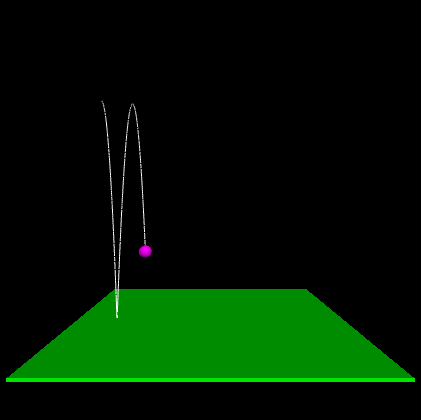
\includegraphics[scale=0.5]{caidalibre}
    \caption{Movimiento parábolico con rebote}
    \label{fig:caidalibre}
  \end{figure}

\end{frame}


\begin{itemize}
\item[\textbf{Ejemplo:}] \textbf{Una bola con resistencia de aire despreciable: 2D, Fuerza constante}
Una bola de masa 500~g está inicialmente en el suelo, en una ubicación $(0,0,0)\ $m. La bola es entonces pateada con una velocidad inicial $(4,7,0)\ $m/s.
\begin{enumerate}
\item ¿Donde estará la bola medio segundo después?
\label{item:8}
\item ¿En que tiempo la bola golpeará el piso?
\label{item:9}
\end{enumerate}
Haga la aproximación que la resistencia del aire es despreciable.


\item[\textbf{Solución:}] Sistema: bola\\
Entorno: Tierra\\
Diagrama de cuerpo libre: ver figura\\
Tiempo inicial: El instante en que el pie ya no esta en contacto con la bola
\begin{itemize}
\item[~\ref{item:8}]
Después de medio segundo
\begin{align}
  x_f=&x_i+v_{xi}\Delta t\nonumber\\
  =&0+(3\ \text{m/s})(0.5\ \text{s})=1.5\ \text{m}
\end{align}
\begin{align}
  y_f=&y_i+v_{yi}\Delta t-\frac{1}{2}g \Delta t^2\nonumber\\
=& 0+(7\ \text{m/s})(0.5\ \text{s})-\frac{1}{2}(9.8\ \text{N/kg})(0.5\ \text{s})^2=2.275\ \text{m}
\end{align}
El vector final de desplazamiento es
\begin{align}
  \mathbf{r}_f=(1.5,2,2,75,0)\ \text{m}
\end{align}
Comprobación: Las unidades son correctas, y la bola se ha movido en la dirección apropiada
\item[~\ref{item:9}] Tiempo final: El instante justo antes de que la bola golpee el piso. En ese instante sabemos que $y_f=0$, de modo que podemos encontrar $\Delta t$
  \begin{align}
    0=0+v_{yi}\Delta t-\frac{1}{2}g\Delta t^2
  \end{align}
  \begin{align}
 \Delta t(v_{yi}-\frac{1}{2}g\Delta t)=0   
  \end{align}
  \begin{align}
    \Delta t=&0 &\text{o}\qquad v_{yi}-\frac{1}{2}g\Delta t=&0
  \end{align}
El segundo valor es el tiempo cuando la bola retorna al suelo
\begin{align}
  \Delta t=&\frac{2 v_{yi}}{g}\nonumber\\
=&\frac{2(7\ \text{m/s})}{9.8\ \frac{N}{Kg}}=1.43\ \text{s}
\end{align}
\end{itemize}

\end{itemize}

\subsection{Gráficos de movimiento}

Para el anterior ejemplo {Movimiento en $x$}
\begin{frame}
\begin{figure}
  \centering
  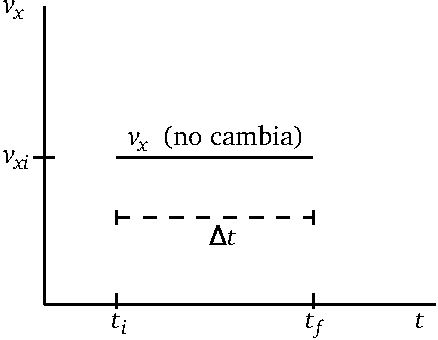
\includegraphics[scale=0.9]{parabgraph1} 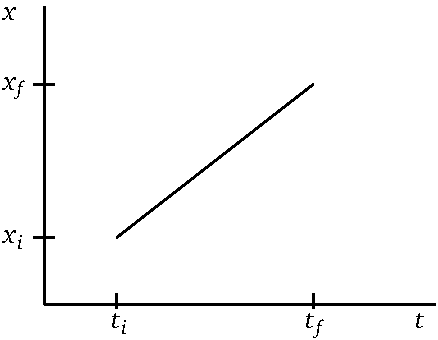
\includegraphics[scale=0.9]{parabgraph2}
  \caption{Movimiento bola}
  \label{fig:parabgraph1}
\end{figure}
\end{frame}

\begin{frame}
\begin{figure}
  \centering
  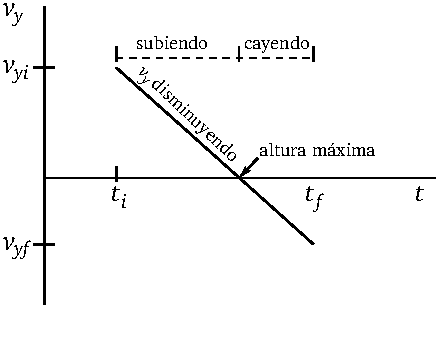
\includegraphics[scale=0.9]{parabgraph3}  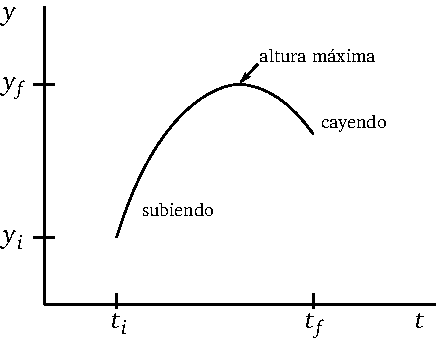
\includegraphics[scale=0.9]{parabgraph4}
  \caption{Movimiento bola}
  \label{fig:parabgraph3}
\end{figure}
\end{frame}

\begin{frame}
\begin{figure}
  \centering
  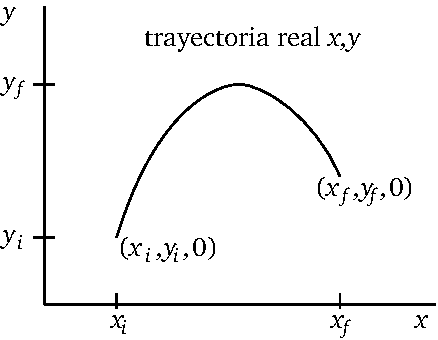
\includegraphics{parabgraph5}
  \caption{Movimiento bola}
  \label{fig:parabgraph3}
\end{figure}
\end{frame}

\subsection{Ejemplos movimiento parbólico}

\begin{inprogress}
  Ejemplo notas Kowalski 3-13
\end{inprogress}

\begin{itemize}
\item[\textbf{Ejemplo:}] Una piedra es lanzada hacia arriba desde lo alto de un edificio con una velocidad inicial de 20 m/s directamente hacia arriba. El edificios tiene 50 m de alto, y la piedra falla en golpear el edificio en su camino hacia abajo.
  \begin{enumerate}
  \item \textquestiondown Qu\'e tiempo le toma a la piedra alcanzar su m\'axima altura?
    \begin{align}
      v(t)=v_0-gt\,.
    \end{align}
    A la altura m\'axima $v=0$, y con $v_0=+20$ m/s
    \begin{align}
      t_{\text{max}}=&\frac{v_0}{g}\nonumber\\
      =&\frac{20}{9.8}\ s\nonumber\\
      \approx&2.04\ s
    \end{align}
  \item \textquestiondown Cual es la m\'axima altura desde la base del edificio?:\\
    Tomando el origen de coordenadas en la base del edificio:
    \begin{align}
      y_{\text{max}}=&y_0+v_o t-\frac{1}{2}g t^2\nonumber\\
      \approx&50+20\timesm2.04-\tfrac{1}{2}\timesm9.8\timesm(2.04)^2\nonumber\\
      \approx&70.4\ \text{m}\,,
    \end{align}
  \item \textquestiondown Cual es el tiempo necesario para que la piedra retorne al nivel de la torre?\\
    \begin{align}
      t_{\text{torre}}=2t_{\text{max}}\approx4.08\ \text{s}\,.
    \end{align}
  \item \textquestiondown La velocidad a ese instante?\\
    \begin{align}
      v=&v_0-gt\nonumber\\
      \approx&20-9.8\timesm4.08\\
      v_{\text{torre}}\approx&-20\ \text{m/s}\,,
    \end{align}
    La misma magnitud que la velocidad inicial pero con direcci\'on opuesta. La velocidad incial estar\'\i a representada por un vector $\mathbf{v}_0$: $\uparrow$, mientras que $\mathbf{v}_{\text{torre}}:$ $\downarrow$.
  \item \textquestiondown Cual es la velocidad y posici\'on (desde la base del edificio) despu\'es de $t=5\ \text{s}$?
    \begin{align}
      v(5)\approx 20-9.8\timesm5\approx-29.0\ \text{s}\,.
    \end{align}
    \begin{align}
      y(5)\approx50+20\timesm5-\tfrac{1}{2}\timesm9.8\timesm5^2\approx27.5\ \text{m}\,.
    \end{align}
  \item \textquestiondown Cual es la velocidad y el tiempo cuando la piedra golpea el piso?
    \begin{align}
      y_0=&50\ \text{m} & y_{\text{final}}=0\nonumber\\
      \mathbf{v}_0=&20\hat{\mathbf{j}}\ \text{m/s} & \\
    \end{align}

    \begin{align}
      v^2=&v_0^2-2g(y_{\text{final}}-y_0)\nonumber\\
      =&v_0^2-2g(0-y_0)\nonumber\\
      \approx&20^2+2\timesm9.8\timesm 50\,,
    \end{align}
de donde
\begin{align}
  \mathbf{v}_{\text{final}}=-37.1 \hat{\mathbf{j}}\ \text{m/s}\,.
\end{align}
\begin{align}
  t_{\text{final}}=&(v_0-v_{\text{final}})/g\nonumber\\
  \approx&(20+37.1)/9.8\approx5.83\,s
\end{align}
  \end{enumerate}
\end{itemize}

\subsection{Movimiento parabólico completo}

En un movimiento parabólico completo, donde un cuerpo es lanzado desde
el suelo con cierta velocidad inicial y retorna al suelo sobre una
superficie horizontal, podemos especificar el alcance $R$ y la altura
máxima $y_{\text{max}}$ en términos de la rapidez inicial, $v$, y el
ángulo de lanzamiento $\theta$. Como
$\mathbf{r}_i=(x_i,y_i,0)=(0,0,0)$, tenemos
  \begin{enumerate}
  \item Altura máxima: se obtiene de la condición $v_y=0$. Reemplazando en la ec.~\eqref{eq:33}
    \begin{align}
      0=v_{yi}-g\Delta t\,,
    \end{align}
de modo que para alcanzar $y_{\text{max}}$ el cuerpo se tarda
\begin{align}
  \label{eq:34}
  \Delta t=\frac{v_{yi}}{g}\,.
\end{align}
Reemplazando \eqref{eq:34} en \eqref{eq:32}, tenemos
\begin{align}
  y_{\text{max}}=&v_{yi}\frac{v_{yi}}{g}-\frac{1}{2}g\frac{v_{yi}^2}{g^2}\nonumber\\
  =&\frac{v_{yi}^2}{g}-\frac{1}{2}\frac{v_{yi}^2}{g}\nonumber\\
  =&\frac{1}{2}\frac{v_{yi}^2}{g}\,.
\end{align}
En términos de la rapidez inicial y el ángulo de lanzamiento tenemos
\begin{align}
  y_{\text{max}}=\frac{v^2}{g}\sin^2\theta\,,
\end{align}
La mayor de las alturas máximas se obtiene para $\theta=\pi/2=90^\circ$, es decir cuando la velocidad inicial está toda en $y$.
\item Alcance: se obtiene de la condición: $y=0$. Reemplazando en la ec.~\eqref{eq:32}
  \begin{align}
    0=&v_{yi}\Delta t-\frac{1}{2}g\Delta t^2\nonumber\\
    =&\Delta t(v_{yi}-\frac{1}{2}g\Delta t)\to
    \begin{cases}
      \Delta t=0 & x=0\\
      v_{yi}-\frac{1}{2}g\Delta t=0 & x=R\\
    \end{cases}
\,,
  \end{align}
de modo que para alcanzar $R$ el cuerpo se tarda
\begin{align}
 \label{eq:35}
  \Delta t=\frac{2v_{yi}}{g}\,.
\end{align}
Reemplazando \eqref{eq:35} en \eqref{eq:32}, tenemos
\begin{align}
  R=&v_{xi}\frac{2v_{yi}}{g}\nonumber\\
  =&\frac{2v_{xi}v_{yi}}{g}\,.
\end{align}
En términos de la rapidez inicial y el ángulo de lanzamiento tenemos
\begin{align}
  R=&\frac{2v^2}{g}\cos\theta\sin\theta\,,
\end{align}
y usando
\begin{align}
  \sin(\alpha+\beta)=\sin\alpha\sin\beta+\cos\alpha\sin\beta
\end{align}
tenemos que $\sin(2\theta)=2\sin\theta\cos\theta$, y
\begin{align}
  R=\frac{v^2}{g}\sin(2\theta)\,,
\end{align}
de modo que el alcance máximo se obtiene para $\theta=\pi/4=45^\circ$,
es decir, cuando las componentes de la velocidad inicial se reparten
por igual en $x$ y $y$.
  \end{enumerate}



\begin{inprogress}
  Copiar ejemplo de tanque en movimiento disparando verticalmente hacia arriba.
\end{inprogress}

\begin{itemize}
\item[\textbf{Ejemplo}] \textbf{El mono}\\
Un mono se suelta de un \'arbol a una altura $h_0$ en el mismo instante en el que le disparan. \textquestiondown Con que \'angulo se debe apuntar al mono para atinarle?
  \begin{align}
    y_{\text{bala}}(t)=&(v_0\sin\alpha)t-\tfrac{1}{2}g t^2\nonumber\\
    y_{\text{mono}}(t)=&h_0-\tfrac{1}{2}g t^2\,.
  \end{align}
Supongamos que en el punto $P$: $y_{\text{bala}}=y_{\text{mono}}$. Entonces
\begin{align}
  v_0 t_P\sin\alpha=&h_0\,.
\end{align}
Sea $D$ la distancia horizontal recorrida en el tiempo $t_P$. Como $v_x=v_0\cos\alpha=\text{cte}$, entonces
\begin{align}
  (t_Pv_0\cos\alpha)\frac{\sin\alpha}{\cos\alpha}=h_0\,,
\end{align}
de modo que
\begin{align}
  \tan\alpha=\frac{h_0}{D}\,.
\end{align}
Entonces, para atinarle al mono, se debe apuntar directamente a \'el.

\item[\textbf{Ejercicio}]Calcula la m\'\i nima distancia para que una bala disparada con una velocidad de $3\ \text{m/s}$, apuntada a la cabeza de un mono de $0.5\ $m de altura y a $10\ $m del suelo y que se quede quieto, pase justo por debajo de sus pies. (Respuesta: $95.3\ $m)
\end{itemize}





\begin{borrar}
En una dimensi\'on es establecida por la ecuaci\'on
\begin{align}
  \label{eq:2ndlaw1d}
  a=\frac{F}{m}\,,
\end{align}
donde $F$ es la fuerza actuando sobre un cuerpo de masa $m$. 

\begin{itemize}
\item[\textbf{Ejemplo:}] Establezca cual es la fuerza asociada a la ca\'\i da libre.

Para obtener la ecuaci\'on de movimiento:
\begin{align}
  \frac{d^2y(t)}{dt^2}=-g\,,
\end{align}
se requiere que un cuerpo en ca\'\i da libre de masa $m$ sufra una fuerza:
\begin{align}
  F=-m\,g\,.
\end{align}

\end{itemize}

En general, la ecuaci\'on de movimiento en una dimensi\'on puede escribirse como
\begin{align}
  \frac{d^2x(t)}{dt^2}-\frac{F(x)}{m}=0\,.
\end{align}

La ecuaci\'on~(\ref{eq:2ndlaw1d}) puede escribirse en una forma m\'as familiar como
\begin{align}
  F=m\,a\,.
\end{align}
En el sistema internacional de unidadades (SI), la unidad de Fuerza es el \emph{Newton} (N), la unidad de masa es el \emph{Kilogramo} (kg), y la aceleraci\'on es en metros por segundo al cuadrado ($\metre\per\second\squared$):
\begin{align}
  F=&m\,a\nonumber\\
&[\kilo\gram]
\left[\frac{\meter}{\second\squared}\right]\nonumber\\
=&\newton\,.
\end{align}
La masa es la resistencia de un cuerpo a cambiar su estado de movimiento.

En t\'erminos vectoriales, concluimos que la fuerza total $\mathbf{F}$ en un cuerpo de masa $m$ es
\begin{align}
  \mathbf{F}=\sum_i \mathbf{F}_i\,.
\end{align}
Si $\mathbf{a}$ es la aceleraci\'on neta, y $\mathbf{a}_i$ la aceleraci\'on debida a $\mathbf{F}_i$ solamente, entonces tenemos
\begin{align}
  \mathbf{F}=&\sum_i \mathbf{F}_i\nonumber\\
  =&\sum_i m\mathbf{a}_i\nonumber\\
  =&m\sum_i \mathbf{a}_i\nonumber\\
  =&m\mathbf{a}\,,
\end{align}
o
\begin{align}
  \label{eq:fma}
  \mathbf{F}=m\mathbf{a}\,.
\end{align}
Esta es la segunda Ley de movimiento de Newton. Las fuerzas surgen de las \emph{interacciones} entre dos sistemas. Por esto raz\'on, en cuanto aislemos un cuerpo lo suficiente de sus alrededores, esperaremos que el cuerpo se mueva uniformemente en un sistema inercial.

Cuando se define cuerpo aislado, el aislamiento significa eliminar las interacciones. Usualmente, para aislar un cuerpo es suficiente moverlo lo suficientemente lejos de todo lo dem\'as. En tal caso las interacciones pueden reducirse tanto como uno desee.
  
\end{borrar}


\begin{itemize}
\item[\textbf{Ejemplo}:] Para el diagrama en la figura~\ref{fig:forces}, calcule la fuerza resultante.
  \begin{figure}
    \centering
    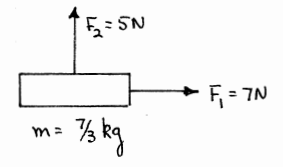
\includegraphics[scale=0.7]{forces}
    \caption{Fuerza resultante}
    \label{fig:forces}
  \end{figure}

Se escoge un sistema de coordenadas tal que
\begin{align}
  \mathbf{F}_1=&7\hat{\mathbf{i}}+0\hat{\mathbf{j}}\nonumber\\
  \mathbf{F}_2=&0\hat{\mathbf{i}}+5\hat{\mathbf{j}}\,.
\end{align}
Entonces
\begin{align}
  \mathbf{F}_R=\mathbf{F}_1+\mathbf{F}_2=
  7\hat{\mathbf{i}}+5\hat{\mathbf{j}}\,.
\end{align}
La aceleraci\'on, que esta en la misma direcci\'on que la fuerza esta dada por
\begin{align}
  \mathbf{a}=\frac{\mathbf{F}_R}{m}=\frac{7\hat{\mathbf{i}}+5\hat{\mathbf{j}}}{7/3}=3\hat{\mathbf{i}}+\frac{15}{7}\hat{\mathbf{j}}\,.
\end{align}

\item[\textbf{Ejemplo:}] Un disco plano de masa $m=2\kilo\gram$, se desliza sobre un lago congelado con una velocidad inicial de $v=5\meter\per\second$. La fuerza de fricci\'on tiene un valor constante de $f=4\newton$ opuesta al movimiento. \textquestiondown cuan lejos avanza el disco antes de detenerse?

Escogiendo apropiadamente el sistema de coordenadas, tenemos:
\begin{align}
  -f \hat{\mathbf{i}}=m\mathbf{a}\,,
\end{align}
de donde
\begin{align}
  \mathbf{a}=-\frac{f}{m}\hat{\mathbf{i}}=\frac{-4\newton}{2\kilo\gram}\hat{\mathbf{i}}=\unit{-2\hat{\mathbf{i}}}{\meter\per\second\squared}\,.
\end{align}
De la cinem\'atica del problema tenemos
\begin{align}
  v_f^2-v_0^2=2 g x\,.
\end{align}
Cuando el disco se detiene $\mathbf{v}_f=0$, de modo que
\begin{align}
  -v_0^2=&2ax\nonumber\\
  x=&-\frac{v_0^2}{2a}=\unit{6.25}{\meter}\,.
\end{align}


\end{itemize}

\subsection{Tercera Ley de Newton}
Las fuerzas siempre aparecen en pares: si un cuerpo $b$ ejerce una fuerza $\mathbf{F}_a$ en un cuerpo $a$, entonces debe haber otra fuerza $\mathbf{F}_b$ actuando en el cuerpo $b$, debido al cuerpo $a$, tal que
\begin{align}
  \mathbf{F}_b=-\mathbf{F}_a\,.
\end{align}
En otras palabras
\begin{align}
  \text{acci\'on}=-\text{reacci\'on}\,:
\end{align}
Si un cuerpo aislado sufre una aceleraci\'on y no podemos encontrar un objeto externo que sufre una aceleraci\'on igual pero opuesta, entonces estaremos en problemas. Un ejemplo mas típico de un par acción-reacción es el de dos patinadores sobre hile intercambiando una pelota.

La segunda ley $\mathbf{F}=d\mathbf{p}/dt$, se mantiene cierta sólo en sistemas inerciales.

En general, las leyes de Newton se mantienen s\'olo en sistemas inerciales. Entonces ¿como se puede decidir o no si un sistema es inercial?:
\begin{itemize}
\item Tome un cuerpo libre.
\item Si este permanece en un estado de movimiento uniforme, entonces se esta en un sistema inercial.
\end{itemize}

La tierra es b\'asicamente un sistema inercial en el cual la aceleración centrípeta debida a la rotación en el Ecuador es de $0.34\meter\per\second\squared$

La estructura y el comportamiento del Universo entero puede ser descrito por la acción de cuatro fuerzas fundamentales descritas en la tabla~\ref{tab:forces}
\begin{table}
  \centering
  \begin{tabular}{l|cc|r}
    &Rango& Intensidad&Mediador\\\hline
Fuerza fuerte (n\'ucleos hadr\'onicos) & $10^{-15}\meter$ &1 &gluones\\
Fuerza electromagn\'etica (cargas) & $\infty$ & $10^{-2}$ & fot\'on\\
Fuerza d\'ebil &$10^{-17}\meter$&$10^{-13}$ (isosp\'\i n)& $W^\pm,\ Z^0$\\
Fuerza gravitacional (masas)&$\infty$& $10^{-38}$& gravit\'on\\
  \end{tabular}
  \caption{Fuerzas fundamentales. La intensidad se mide con respecto a la fuerza entre dos protones separados $10^{-15}\meter$}
  \label{tab:forces}
\end{table}



\section{Aplicaciones de las leyes de Newton}
El método para resolver un problema de din\'amica, consiste en
\begin{itemize}
\item Escoja un sistema, consistiendo de una porción del Universo. El resto del Universo es llamado el entorno.
\item Haga una lista de los objetos del entorno que ejercen fuerzas significativas sobre el sistema escogido. 
\item Haga un diagrama mostrando las fuerzas externas ejercidas por los objetos del entorno sobre el sistema. Esto es llamado un ``diagrama de cuerpo libre'' en el cual el efecto del entorno sobre el sistema es indicado con flechas que representan las fuerzas externas.
\item Establezca los tiempos iniciales y finales
\item Establezca las ecuaciones de movimiento de cada cuerpo
\item Identifique las fuerzas de acci\'on--reacci\'on
\item Establezca las condiciones de ligadura.
\item Comprueba unidad, compruebe la lógica de su respuesta (dirección del moméntum, cambio en la magnitud del moméntum) basado en la situación física.
\end{itemize}

 

Para ilustrar estos pasos, considere el diagrama de bloques mostrado en la figura~\ref{fig:blocks}, los cuales se encuentran en reposo. Encuentre la Fuerza ejercida por el bloque $B$ sobre el $A$, y la fuerza normal de la superficie sobre el bloque $B$.


 $\mathbf{F}_A$ es la fuerza que ejerce el bloque $A$ sobre el bloque $B$, mientras que $\mathbf{F}_B$ es la fuerza que ejerce el bloque $B$ sobre $A$. De acuerdo a la tercera ley de Newton
\begin{align}
  \mathbf{F}_B=\mathbf{F}_A\,.
\end{align}
Note que la tercera ley de Newton nunca relaciona dos fuerzas actuando sobre el mismo cuerpo; las fuerzas de dos cuerpos diferentes son las que est\'an involucradas en la tercera ley. En la figura \ref{fig:blocks}: $\mathbf{N}$ representa la fuerza normal que ejerce el piso sobre el bloque $B$, mientras que $\mathbf{W}_A$ y $\mathbf{W}_B$ representan los pesos de los bloques $A$ y $B$ respectivamente. 


\begin{figure}
  \centering
  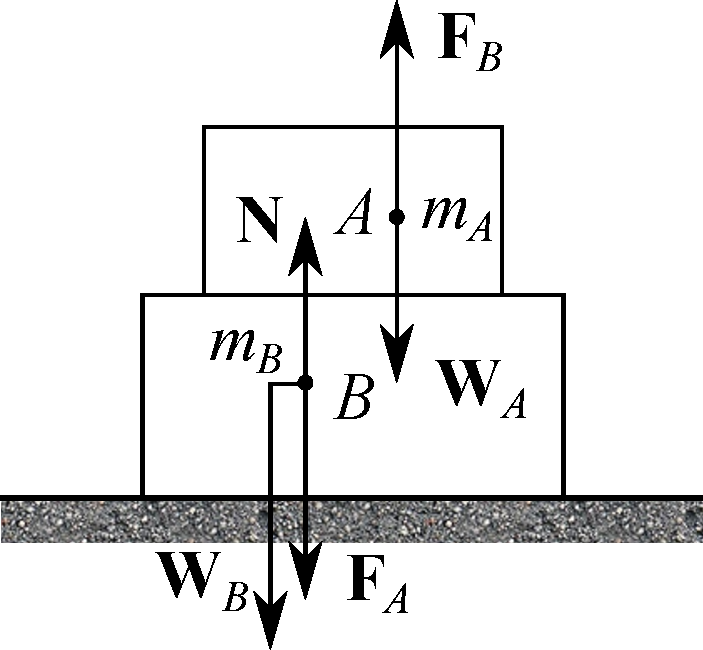
\includegraphics[scale=0.7]{blocks}
  \caption{Diagrama de fuerzas}
  \label{fig:blocks}
\end{figure}

Completando el problema de los dos bloques sobre la superficie tenemos, en la direcci\'on $\hat{\mathbf{j}}$:
\begin{align}
  \text{Ecuaciones de movimiento}&
  \begin{cases}
F_B-W_A=m_A a_A\\
N-F_A-W_B=m_B a_B\\
  \end{cases}\nonumber\\
\text{Tercera ley de Newton}\quad &F_A=F_B\nonumber\\
\text{Constraint equations}&
\begin{cases}
a_A=0\\
a_B=0\\  
\end{cases}
\end{align}
Solucionando las ecuaciones encontramos
\begin{align}
  F_B=&F_A=W_A\nonumber\\
  N=&W_A+W_B\,.
\end{align}
El objetivo principal de este ejemplo es ayudar a distinguir entre la fuerza que se aplica a un objeto 


\begin{itemize}
\item[\textbf{Ejemplo:}] Dos astronautas inicialmente en reposo en el espacio libre, tiran de ambos lados de una cuerda. La fuerza con la que el astronauta $A$ puede tirar de la cuerda, $F_A$ es mayor que la del astronauta $B$, $F_B$. Sus masas son $M_A$ y $M_B$ y la masa de la cuerda es despreciable. Encuentre el movimiento de la cuerda

Sistema: Cuerda

Entorno: Astronautas

Diagrama de cuerpo libre: (pendiente)

Ecuación de movimiento para la cuerda:
\begin{align}
  {F}_{A'}=&F_{A}\nonumber\\
  {F}_{B'}=&F_{B}
\end{align}

\begin{align}
  F_{A'}-F_{B'}=&m_{\text{cuerda}} a_{\text{cuerda}}\nonumber\\
  F_{A}-F_{B}=&m_{\text{cuerda}} a_{\text{cuerda}}\nonumber\\
\approx&0\times a_{\text{cuerda}}\nonumber\\
=&0\,,
\end{align}
de donde
\begin{align}
  F_A=F_B
\end{align}
y no hay movimiento neto de la cuerda.
\end{itemize}

\section{Ingredientes de problemas de dinámica}

\subsection{El peso}
Como hemos visto en la definción de la segundo Ley de Newton, la masa es una medidad de la resistencia que un cuerpo ofrece a los cambios en su velocidad. En la expresión para la segunda Ley de Newton con masa constante
\begin{align}
  \mathbf{F}=m_I \mathbf{a}\,,
\end{align}
$m_I$ es la masa inercial. Es el valor númerico que se obtiene al tirar un cuerpo desplazandose en una superficie sin fricción con un dinanómetro. Si simplemente se sostiene el mismo peso con un dinanómetro sobre la superficie de la tierra, obtenemos la masa gravitacional
\begin{align}
  \mathbf{F}=&m_G\mathbf{g}&\text{donde}\qquad \mathbf{g}\approx(0,-9.8,0)\ \text{m}/\text{s}^2\,,
\end{align}
Numericamente el valor de ambas masas coinciden $m=m_I=m_G$. La proporcionalidad entre masa inercial y masa gravitacional es una hipótesis en la Mecánica Newtoniana, pero es un resultado de la Teoría General de la Relatividad. Definimos entonces el peso de una partícula como el valor de la masa gravitacional por la aceleración gravitacional
\begin{align}
  |\mathbf{W}|=mg\,.
\end{align}

Hay que tener en cuenta sin embargo, que las básculas realmente miden es la fuerza normal

\subsection{Fuerza normal}
Para que un cuerpo se mantenga sobre una superficie se requiere que su peso sea compenzado por una fuerza igual y en sentido opuesto ejercida por la superficie sobre el cuerpo. Dicha fuerza se llama la fuerza normal de la superficie y se denota con la letra $\mathbf{N}$

%introducir discusion de fuerzas interatómicas

En general la fuerza normal debe incluir la presión atmosférica. Para una cuerpo con una area $A$ expuesta a la atmosféra sobre una superficie horizontal, se tendría 
\begin{align}
 N=mg+P_a A\,, 
\end{align}
donde $P_a$ es la presión atmosférica. 
\begin{itemize}
\item[\textbf{Ejemplo}] \textbf{Tortuga dentro de un ascensor}. Suponga que una tortuga, de masa $m$, esta sobre una báscula dentro de un ascensor que se mueve verticalmente con una aceleración de magnitud $a_y$. Calcule la fuerza normal sobre la tortuga ejercida por la báscula. El diagrama de fuerza se muestra en la Figura (pendiente). 

La ecuación de movimiento en la dirección $y$ es (suponiendo una aceleración en la dirección $y$ positiva), con $\mathbf{N}=(0,N,0)$, $\mathbf{F}_{\text{grav}}=(0,-mg,0)$, y $\mathbf{a}=(0,a_y,0)$
\begin{align}
  N-mg=m a_y\,,
\end{align}
de modo que
\begin{align}
  N=m(g+a_y)
\end{align}
Si $a_y=0$, $N=mg$, y la báscula entrega la masa correcta para la
tortuga, sin embargo para una $a_y$ diferente de cero, la báscula
registra una ``masa'' que puede ser mayor o menor que $m$. Para
$a_y=-g$, es decir, que el ascensor se encuentra en caída libre hacia
la superficie de la tierra $N=0$, y la báscula registra un peso cero
para la tortuga. De hecho en esta situación la tortuga se encuentra en
estado de ingravidez: Un sistema cerrado (el ascensor con su contenido
interior) en caída libre en un campo gravitacional constante, es
indistinguible de un sistema con gravedad cero, es decir, el mismo
ascensor en el espacio exterior alejado de cualquier otro cuerpo.
\end{itemize}

\subsection{Cuerdas ideales}
\begin{itemize}
\item[\textbf{Ejemplo}] \textbf{Cuerda no ideal}
\end{itemize}

\subsection{Poleas ideales}

\subsection{Aplicaciones en entornos sin fricción}







\begin{itemize}
\item[\textbf{Ejemplo:}] Tres vagones de masa $M$ están halados con una fuerza $F$ por una locomotora. Despreciando las fuerza de fricción con los rieles, encuentre las fuerzas en cada carro.
  \begin{enumerate}
  \item Sistema: Los tres vagones\\
  Entorno: los rieles y el aire\\
Diagrama: (pendiente)
  \begin{align}
    F=3M a\,,
  \end{align}
de donde
\begin{align}
  a=\frac{F}{3M}
\end{align}
\item Sistema: Primer vagón\\
Entorno: Segundo vagón, rieles, aire\\
Diagrama: (pendiente)

  \end{enumerate}
\end{itemize}
\section{Fricci\'on}

\subsection{Fricci\'on din\'amica}
El coeficiente de fricci\'on tiene que ser menor que 1 porque de lo contrario los cuerpos se podrían subir por las paredes.


Una discusión acerca de la física de los ferrocarriles puede encontrarse en \url{http://www.jotdown.es/2012/04/el-ferrocarril-ese-gran-desconocido/}.

\begin{table}
   \centering
   \begin{tabular}{|l|c|c|}\hline
    Superficies & $\mu_e$ & $\mu_d$\\\hline
     Acero-Acero & 0.15 & 0.09\\\hline
   \end{tabular}
  \caption{Coeficientes de Fricción}
   \label{tab:coeffric}
\end{table}

\begin{frame}
  \begin{block}%
{Ferrocarriles:} En efecto, el origen del término ferrocarril son los carriles (1) de hierro, aunque hoy en día tanto el carril como la rueda se fabrican de acero porque este material presenta unas características mecánicas más apropiadas. Además de la interesante cualidad de no tener que arreglar pinchazos (festival del humor), la principal ventaja de un transporte basado en la rodadura entre aceros es el bajo coeficiente de rozamiento que permite que un tren circulando a 100 km/h a la deriva en una vía recta y horizontal, recorra unos 10 km sin detenerse. 
  \end{block}
El coeficiente de resistencia de rodado del acero en un riel varía entre 0.0002 y 0.0010\footnote{\url{http://www.tribology-abc.com/abc/cof.htm}} 
\end{frame}



\begin{itemize}
\item[Ejemplo] \textbf{Acero-Acero: Ferrocarriles} Calcule la distancia de frenado de un tren asumiendo que las ruedas dejan de rotar inmediatamente cuando se mueve a 160~Km/h.

Asumiendo que la fuerza de fricción es constante, tenemos una desaceleración constante de
\begin{align}
  a=&-\frac{f_d}{m_{\text{tren}}}=-\frac{\mu N}{m_{\text{tren}}}=-\frac{\mu m_{\text{tren}} g}{m_{\text{tren}}}=
-\mu g\,.
\end{align}
Aplicando las ecuaciones para movimiento a aceleración constante, tenemos que cuando la rapidez final es cero
\begin{align}
  0=v_o+a\Delta t\,,
\end{align}
de modo que
\begin{align}
  \Delta t = -\frac{v_0}{a}=\frac{v_o}{\mu g}\,.
\end{align}
La distancia recorrida desde el inicio del frenado es
\begin{align}
  x=&v_0 \Delta t +\frac{1}{2}a \Delta t^2\nonumber\\
  =&\frac{v_0^2}{\mu g}+\frac{1}{2}(-\mu g)\frac{v_0^2}{(\mu g)^2}\nonumber\\
 =&\frac{v_0^2}{2\mu g}\,,
\end{align}
Para $\mu_d=0.09$, tenemos $x\approx 1100\ $m.

La ley empírica de frenado de trenes es:
\begin{align}
  x=\frac{3}{2}\frac{v_0^2}{|a|}
\end{align}
donde $a$ es la desaceleración del tren, típicamente alrededor de $-2\ \text{m}/\text{s}^2$
\end{itemize}

\section{Problemas resueltos}

\begin{enumerate}
\item  (Tomado de \cite{gabriel}) Se coloca un bloque de masa $m_1$ sobre un bloque de masa $m_2$ (como se muestra en la figura). Los coeficientes de fricción cinético y estático entre los bloques son $\mu_k$ y $\mu_e$ respectivamente. Suponer que no hay fricción entre el bloque de masa $m_2$ y la superficie sobre la cual reposa. Se aplica una fuerza $\mathbf{F}$ horizontal al bloque de masa $m_2$

  \begin{minipage}{0.4\linewidth}
    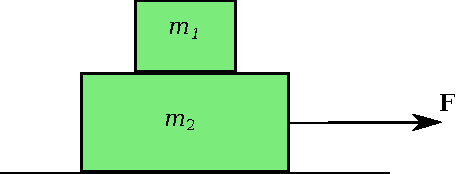
\includegraphics[scale=0.95]{bloques}
  \end{minipage}
  \begin{minipage}{0.6\linewidth}
    \begin{enumerate}
    \item Dibujar todas las fuerzas que actúan sobre cada bloque.
      \label{item:d1a}
    \item Escribir las ecuaciones de movimiento para cada bloque
      \label{item:d1b}
    \item ¿Cuál es la máxima fuerza que puede aplicarse al bloque $m_2$ de modo que los bloques se muevan juntos?
      \label{item:d1c}
    \item ¿Cual es la aceleración cuando se aplica la fuerza máxima?
      \label{item:d1d}
    \item ¿Que distancia recorren los bloques a esa aceleración durante dos segundos?
      \label{item:d1e}
    \item Evalue sus respuestas para $m_1=3\ $Kg, $m_2=5\ $Kg, $\mu_k=0.1$, $\mu_e=0.2$
      \label{item:d1f}
    \end{enumerate}
  \end{minipage}

  \begin{itemize}
  \item[\ref{item:d1b})] Para $m_1$
    \begin{align}
      \label{eq:d11}
      m_1 a_1=&f & N_1-m_1 g=0
    \end{align}
Para $m_2$
\begin{align*}
  m_2 a_2=&F-f & N_2-N_1-m_2g=&0\,.
\end{align*}
    De modo que
    \begin{align*}
      a_1=&\frac{f}{m_1}& a_2=&\frac{F-f}{m_2}\,,
    \end{align*}
    y
    \begin{align*}
      f=\mu m_1 g\,.
    \end{align*}
  \item[\ref{item:d1c})]
    La condición de que los bloques se muevan juntos corresponde a $a_1=a_2$:
    \begin{align*}
      \frac{f}{m_1}=&\frac{F-f}{m_2}\\
      m_2 f =&m_1(F-f)\\
      m_1F =&f(m_1+m_2)\\
      m_1F =&\mu m_1 g(m_1+m_2)\\
      F =&\mu g(m_1+m_2)\,. 
    \end{align*}
    $F$ es máxima cuando $\mu=\mu_e$
    \begin{align*}
      F_{\text{max}}=\mu_e g(m_1+m_2)\,. 
    \end{align*}

    \item[\ref{item:d1d})] La aceleracíon máxima se obtiene de \eqref{eq:d11}:
      \begin{align*}
        a=\frac{f}{m_1}=\mu_e g\,.
      \end{align*}
    \item[\ref{item:d1e})] Para $t=2\second$
      \begin{align*}
        x=&\frac{1}{2}a t^2
      \end{align*}
    \item[\ref{item:d1e})] $F=15.7\newton$, $a=1.96\meter\per\second^2$, $x=3.92\meter$

    \end{itemize}
\end{enumerate}

%%% Local Variables: 
%%% mode: latex
%%% TeX-master: "mecanica"
%%% End: 
